\graphicspath{{introduction/fig/}}

\chapter{Introduction}
\label{chap:introduction}

\section{Background}
The ocean covers 71$\%$ of the earths surface and 80$\%$ of it remains unmapped, unobserved, and unexplored. The ocean produces over half of the air we 
breathe and absorbs 50 times more carbon dioxide than our atmosphere currently does. It regulates our climate and the weather patterns by transporting heat
 from the equator to the poles. It provides sustenance to millions of people around the world.
  % Many medicinal products that help to fight cancer, arthritis
  % and heart disease come from the ocean. Marine transportation makes up a huge portion of global trade, which supports the economies of the world.
   Without 
  the ocean, life as we know it would not be possible and the planet would become uninhabitable.
With that being said 
the rapidly growing global population and consequent resource consumption is impacting 
% the local and 
the global environment 
%  negatively through physical and chemical pollution. 
on a scale that has never been seen before.
% The release of carbon dioxide into the atmosphere contributes to climate change, ocean warming, ocean acidification and the rise in sea
%  levels. When released into the ocean, chemical wastes such agricultural fertilizers result in ocean deoxygenation. Many other forms of pollution such as 
%  untreated waste water and micro and macro plastics have an environmental impact that as of yet is only partially known.

Ocean research has led to our current understanding of the huge role the oceans play in supporting life on this planet. The continuing research and 
exploration of our oceans will aid in assessing the growing negative impact human activity has on the oceans, and by better understanding this impact, 
more effective solutions can be developed. Ocean research requires large amounts of funding and human resources to support it. As of 2015 the United States 
had 4000 ocean science researchers, roughly 50 nationally maintained ocean research vessels and in 2013 had an annual national ocean science expenditure of
$\$12.5$ trillion \cite{Valdes}. These ocean research vessel cost from $\$10000$ to $\$40000$ a day to operate, with the crew itsef being one of the biggest 
expenses\cite{Valdes}.These expenses can increase greatly when research missions to remote areas of the globe are conducted, many of these areas being hard 
or even impossible to access via research vessels. 

Advancements in robotics and the development of unmanned vehicles can help bring down the cost and complexity associated with ocean research missions 
as well as increase the quality of research done. Unmanned sailing vessels(USV) will be able to travel long distances over the ocean, for long periods of 
time, to remote and inaccesable locations and with little power consumption. USV's can be equipped with various high quality sensors 
such as hydrophones that are used in marine research. The integration of solar panels with USV's can further increase the range and 
duration they are capable of.

\section{Problem Statement}
\label{problem_statement}
To design and develop the navigational and control systems for an unmanned sailing vessel that will enable it to sail along a predetermined route with a 
relative degree of accuracy. The route to be travelled is defined by a set of GPS coordinates. 

\section{Objectives}
This section will state the objectives that need to be achieved in order to address the problem statement.

% In order for the navigational systems to work the following objectives need to be achieved. The USV should receive the current GPS coordinates with the 
% standard degree of accuracy associated with the GPS, which is 2.5m. The USV 
% should also be capable of logging the current GPS location as it travels along the route, this is needed to verify successful operation of the USV. 
% Additionally the USV needs to calculate distance between two GPS cordinates accurately in order to determine when it has reached its target location. 
% The USV should be able to calculate bearing given two GPS locations - its current GPS location and its target GPS location.


% In order for the control systems to work the following needs to be achieved.
% The USV needs to be capable of measuring its current bearing to a relative degree of accuracy, this is a requirement for designing the rudder control system. 
% The USV must be capable of determining wind direction relative to itself (apparent wind) and adjust the sail position accordingly. 
% The USV must be able to sail between two predetermined GPS coordinates with minimal deviation between the ideal trajectory and the actual trajectory of the vessel.
% The Vessel should be able to tack into the wind in order to reach a target location. Given that these two objectives have been achieved, the vessel should be
% able to travel between three GPS coordinates such that the travelled path is a triangle.

\begin{enumerate}
  \item Design and develop a digital compass that compensates for tilt.
  % \item Determine and compare the accuracy of heading obtained from a GPS reciever and that from a digital compass.
  \item System must be capable of logging operational data to a micro-SD card.
  \item Design and implement necessary navigational algorithms: Determine distance and bearing between two GPS coordinate.
  \item Design and develop sail control system.
  \item Design and develop rudder control system.
  \item Design and develop software that ensures system in capable of navigating to predetermined waypoints.
  \item Design and implement tacking manuovre into system.
\end{enumerate}

\section{Summary of Work}

\section{Scope}

\section{Report Overview}



% \section{Section heading}

% This is some section with two table in it: Table~\ref{tbl:exemplars} and Table~\ref{tbl:abx_speaker}.

% \begin{table}[!h]
%     \mytable
%     \caption{Performance of the unconstrained segmental Bayesian model on TIDigits1 over iterations in which the reference set is refined.}
%     \begin{tabularx}{\linewidth}{@{}lCCCCC@{}}
%         \toprule
%         Metric     & 1 & 2 & 3 & 4 & 5 \\
%         \midrule
%         WER (\%)                        & $35.4$ & $23.5$ & $21.5$ & $21.2$ & $22.9$ \\
%         Average cluster purity (\%)       & $86.5$ & $89.7$ & $89.2$ & $88.5$ & $86.6$ \\
%         Word boundary $F$-score (\%)         & $70.6$ & $72.2$ & $71.8$ & $70.9$ & $69.4$ \\
%         Clusters covering 90\% of data   & 20             & 13 & 13 & 13 & 13 \\
%         \bottomrule
%     \end{tabularx}
%     \label{tbl:exemplars}
% \end{table}


% \begin{table}[!h]
%     \renewcommand{\arraystretch}{1.1}
%     \centering
%     \caption{A table with an example of using multiple columns.}
%     \begin{tabularx}{0.65\linewidth}{@{}lCCr@{}}
%         \toprule
%         & \multicolumn{2}{c}{Accuracy (\%)} \\
%         \cmidrule(lr){2-3}
%         Model    & Intermediate & Output & Bitrate\\
%         \midrule
%         Baseline & 27.5         & 26.4   & 116 \\
%         VQ-VAE   & 26.0         & 22.1   & 190 \\
%         CatVAE   & 28.7         & 24.3   & 215 \\
%         \bottomrule
%     \end{tabularx}
%     \label{tbl:abx_speaker}
% \end{table}

% \newpage

% This is a new page, showing what the page headings looks like, and showing how to refer to a figure like Figure~\ref{fig:cae_siamese}.

% \begin{figure}[!t]
%     \centering
% %     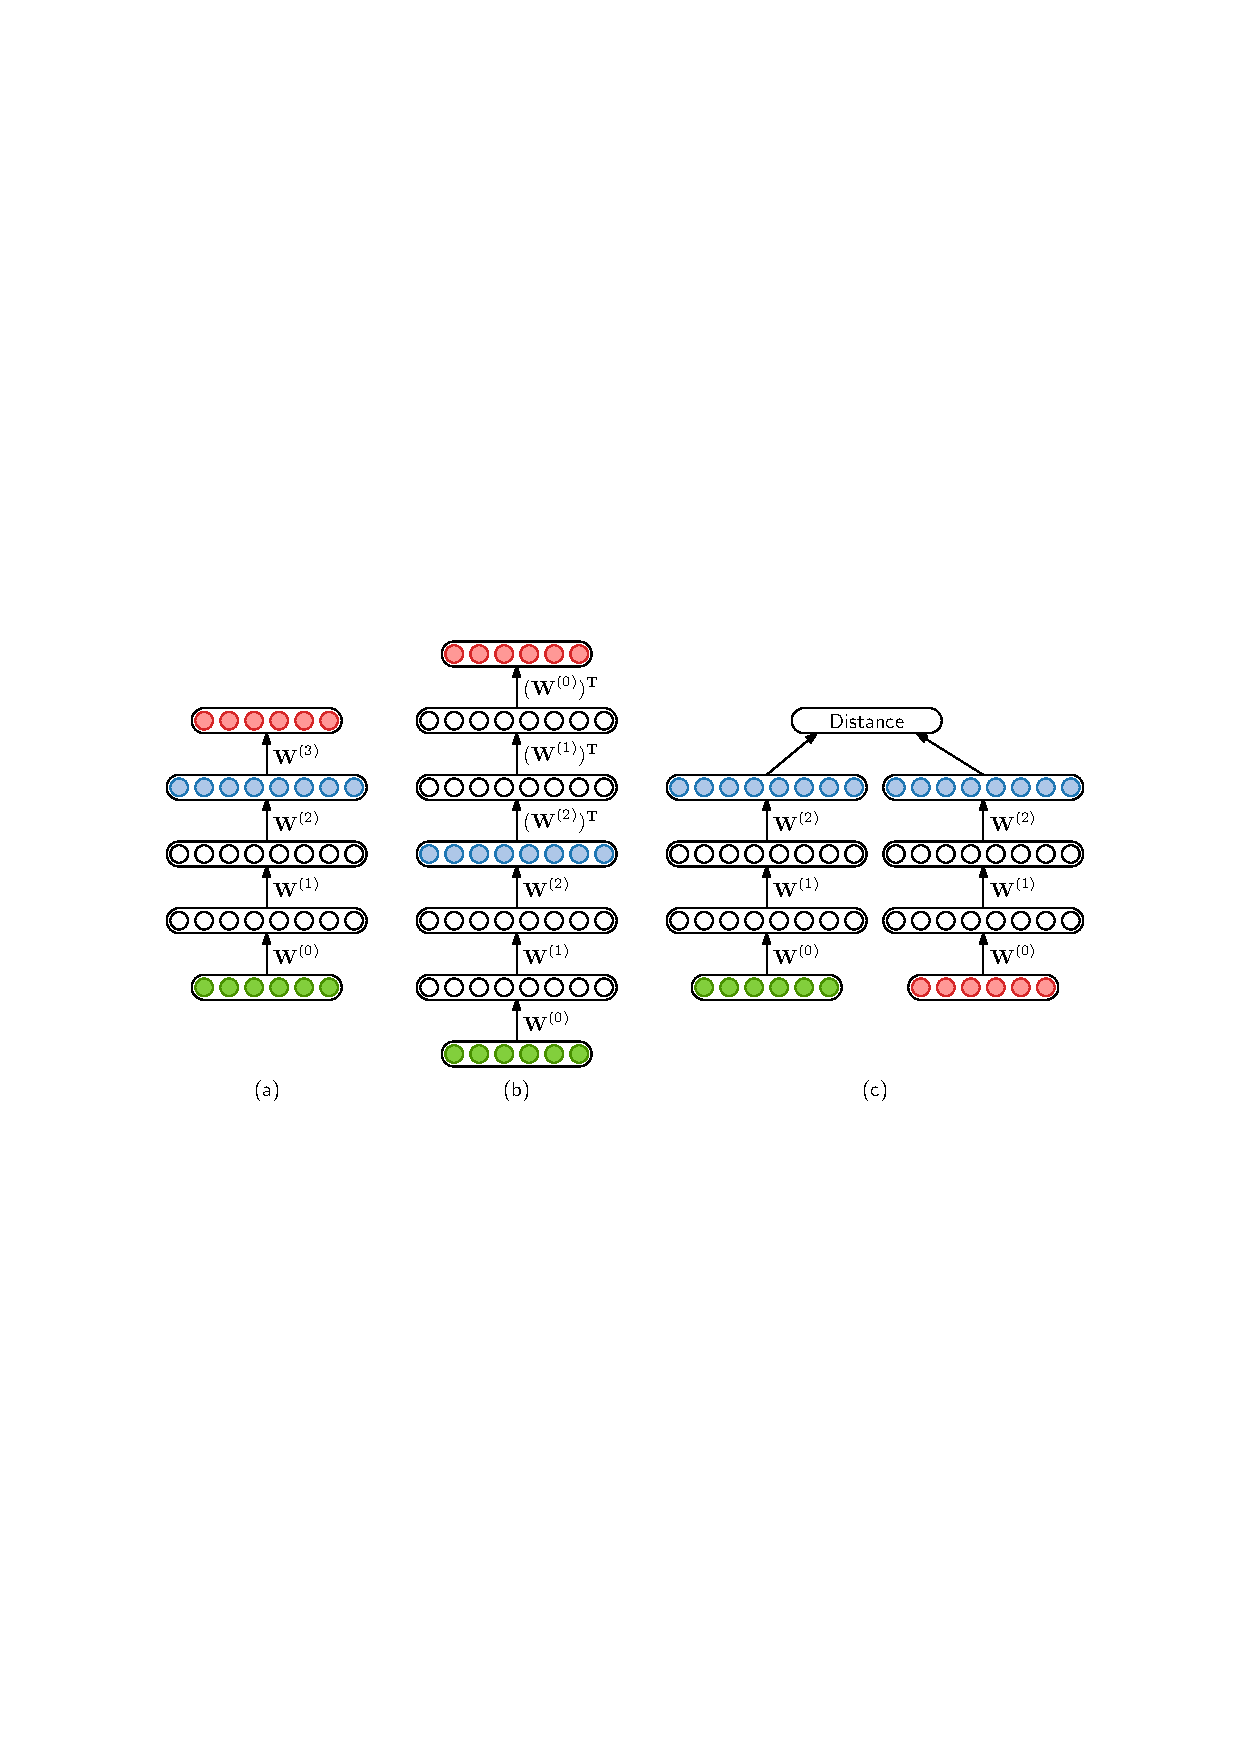
\includegraphics[width=\linewidth]{cae_siamese}
%     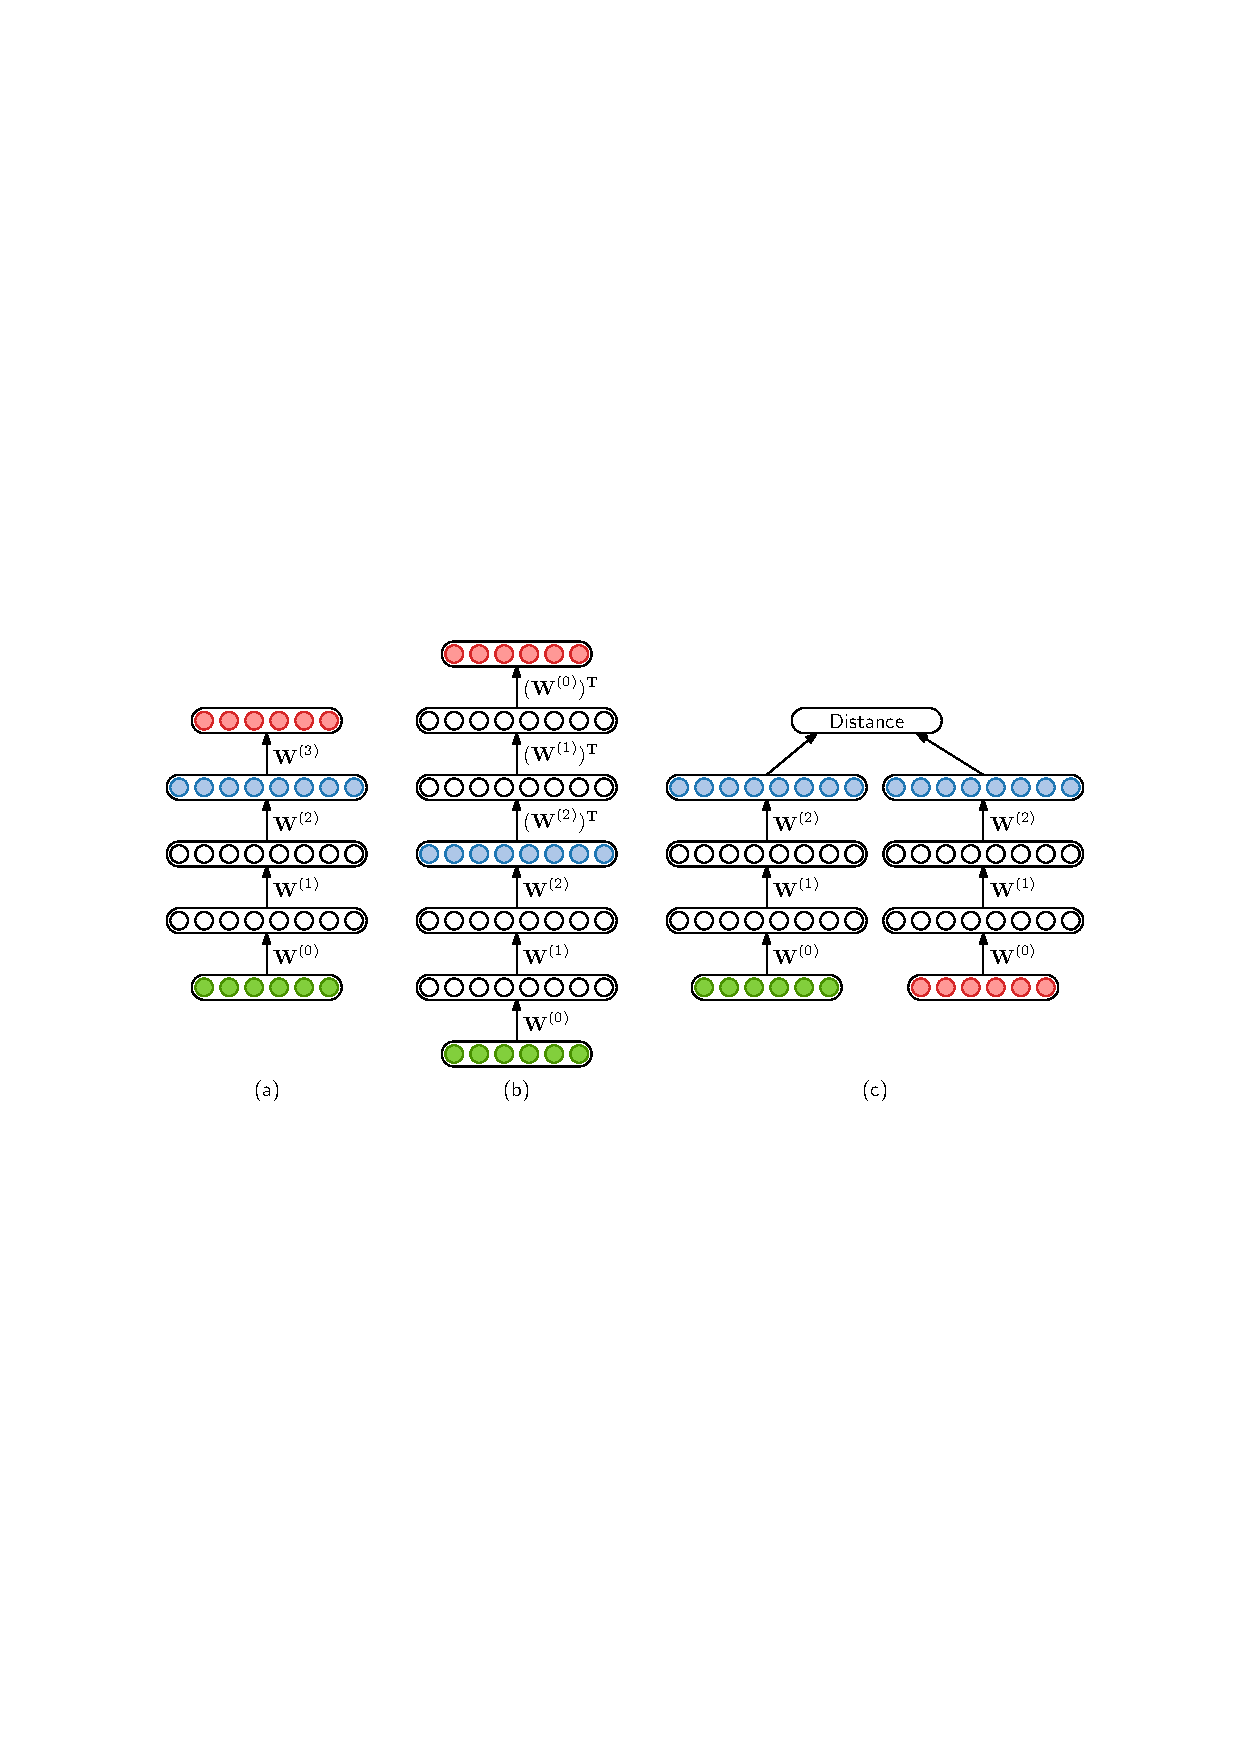
\includegraphics[width=0.918\linewidth]{cae_siamese}
%     \caption[I am the short caption that appears in the list of figures, without references.]{
%     (a) The cAE as used in this chapter. The encoding layer (blue) is chosen based on performance on a development set.
%     (b) The cAE with symmetrical tied weights. The encoding from the middle layer (blue) is always used.
%     (c) The siamese DNN. The cosine distance between aligned frames (green and red) is either minimized or maximized depending on whether the frames belong to the same (discovered) word or not.
%     A cAE can be seen as a type of DNN~\cite{dahl+etal_taslp12}.
%     }
%     \label{fig:cae_siamese}
% \end{figure}


% The following is an example of an equation:
% \begin{equation}
% P(\vec{z} | \vec{\alpha}) = \int_{\vec{\pi}} P(\vec{z} | \vec{\pi}) \, p(\vec{\pi} | \vec{\alpha}) \, \textrm{d} \vec{\pi}
% = \int_{\vec{\pi}} \prod_{k = 1}^K \pi_k^{N_k} \frac{1}{B(\vec{\alpha})} \prod_{k = 1}^K \pi_k^{\alpha_k - 1} \, \textrm{d} \vec{\pi}
% \label{eq:example_equation}
% \end{equation}
% which you can subsequently refer to as~\eqref{eq:example_equation} or Equation~\ref{eq:example_equation}.
% But make sure to consistently use the one or the other (and not mix the two ways of referring to equations).